%ltex: language=de-de
\chapter{Detailierung}
	\begin{figure}[h]
		\centering
		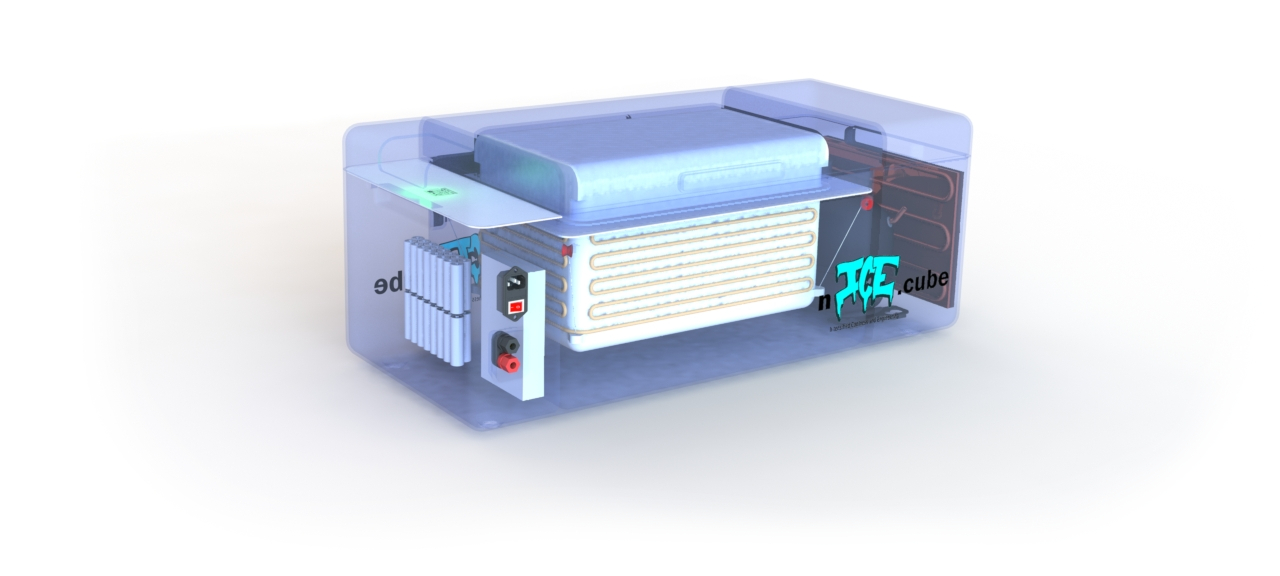
\includegraphics[width=\textwidth]{assets/transp6_edit.JPG}
		\caption{My Caption}
		\label{fig:transparent render}
	\end{figure}
	\section{Stückliste}
		\begin{table}[h]
			\centering
			\caption[Stückliste]{Sückliste.}
			\begin{tabular}[c]{@{}p{.05\textwidth}p{.05\textwidth}p{.1\textwidth}p{.4\textwidth}p{.4\textwidth}@{}}
				\toprule
				Pos. & Menge & Einheit & Benennung & Bemerkung\\
				\midrule
				1&1&Stk.&Ansaugverbindung& \\
				2&4&Stk.&Aramidschnur& \\
				3&1&Stk.&Druckreduzierer& \\
				4&2&Stk.&Durchführung&\\
				5&1&Stk.&Dämpfer&\\
				6&1&Stk.&E-Ink Display& \\
				7&1&Stk.&Ein-/Ausgabepanel& \\
				8&4&Stk.&Elektronik& \\
				9&1&Stk.&Elektronikdeckel& \\
				10&1&Stk.&Gummimanschette& \\
				11&1&Stk.&Hülle&\\
				12&1&Stk.&Kompressor&\textit{CASCADE17-0146Y1}\\
				13&1&Stk.&Kompressordeckel& \\
				14&1&Stk.&Kältemittelverbindung von Verflüssiger& \\
				15&1&Stk.&Kältemittelverbindung zu Verflüssiger& \\
				16&32&Stk.&Li-Ion 18650&8S4P Konfiguration\\
				17&1&Stk.&Reduzierer& \\
				18&1&Stk.&Transportgutbehälter&\\
				19&1&Stk.&Trockner&\\
				20&1&Stk.&Verflüssiger&\\
				21&1&Stk.&Verschlussdfeckel außen&\\
				22&1&Stk.&Verschlussdeckel innen&\\
				23&1&Stk.&DC-Anschluss&Buchse für \SI{4,2}{mm} Laborstecker mit Polschraube (Bipolar)\\
				24&1&Stk.&AC-Anschluss&C14 AC Buchse mit Schalter und Sicherungshalter\\
				\bottomrule
			\end{tabular}
		\end{table}